%calcul de l'age
\newcounter{dateone}%
\newcounter{datetwo}%
\setmydatenumber{dateone}{1982}{05}{23}%
\setmydatenumber{datetwo}{\the\year}{\the\month}{\the\day}%
\FPsub\result{\thedatetwo}{\thedateone}
\FPdiv\myage{\result}{365.2425}

\begin{frame}{Mathieu Leocmach, {\normalsize\FPtrunc\myage{\myage}{0}\myage ~ans}\hfill \hspace{3.5cm}Curriculum}
%photo
\newlength{\totorowidth}%
\newsavebox{\totorobox}%
\savebox\totorobox{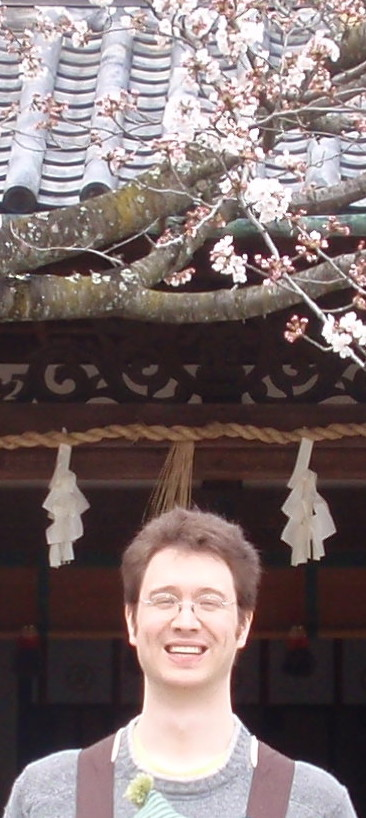
\includegraphics[height=\textheight-\headheight-\footheight-2em]{shikoku.jpg}}%
\settowidth{\totorowidth}{\usebox{\totorobox}}%
%
\begin{columns}[b]
\column{0.7\textwidth}
\begin{description}[2002-05]
\item[2002-05] \nth{1} Master \hfill{\footnotesize Ecole Polytechnique}
\item[2006-08] \nth{2} Master \hfill{\footnotesize Univ. Tokyo}
\item[2008-11] PhD \hfill{\footnotesize Univ. Tokyo}
\item[2011-12] Postdoc \hfill{\footnotesize Univ. Tokyo}
\item[2012-\hfill] Postdoc \hfill{\footnotesize E.N.S. de Lyon}\\
{\footnotesize $\approx$ 60 h/year teaching: 
\begin{itemize}
\item Long ($6\times \SI{8}{\hour}$) physics lab work (Master)
\item Python programming (L3)
\end{itemize}}
\end{description}


\begin{block}{9 articles (5 as first author)\\
\footnotesize 10 invited talks, 4 contributed, 18 posters}
\footnotesize 
\begin{description}[Crystal]
\item[Glass] Nature Commun., J. Chem. Phys., AIP Conf. Proc.
\item[Crystal] Soft Matter, Europhys. Lett.
\item[Oscil. reaction] Chemical Communications
\item[Gel] Phys. Rev. Lett., Macromol. Rapid Commun.
\item[Teaching] Bulletin de l'Union des Physiciens
\hfill\raisebox{0.6\normalbaselineskip}[0pt][0pt]{$\left.\rule{0pt}{1.2\normalbaselineskip}\right\}$ 2014}
\end{description}
\end{block}
\column{\totorowidth}
\usebox{\totorobox}
\end{columns}
\end{frame}

\begin{frame}{PhD: colloidal glass transition}

\begin{block}{Dynamic heterogeneity, candidate structural causes}
\begin{columns}
\column{0.25\textwidth}
\tikzsetnextfilename{dh_perera}\begin{tikzpicture}
\node[inner sep=0] (dh) {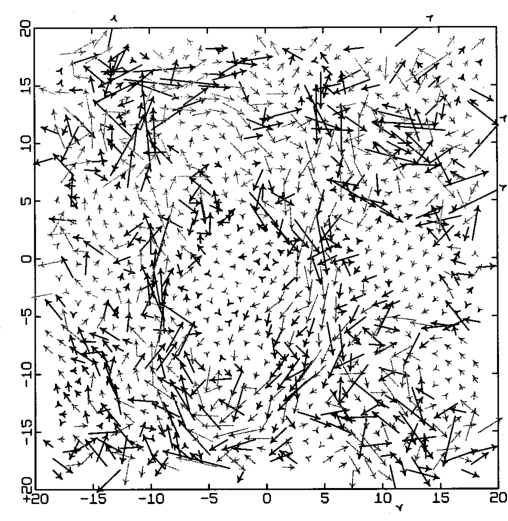
\includegraphics[width=\textwidth]{dh_perera}};
\node[below=0 of dh.north, inner sep=1pt, fill=white, font=\footnotesize\itshape] {Perera 1999};
\end{tikzpicture}
\column{0.6\textwidth}
\begin{enumerate}
\item locally stable structures\\
\tikzsetnextfilename{pentagons}\begin{tikzpicture}[pen/.style={regular polygon, regular polygon sides=5, draw, minimum size=0.4\baselineskip}]
	\node[pen] (base) {};
	\node[pen,anchor=south, rotate=180] at (base.side 3) {};
	\node[pen,anchor=south, rotate=-108] at (base.side 4) {};
\end{tikzpicture}
\hfill {\footnotesize icosahedra}
\item avoided crystal influence\\
\newdimen\radius
\setlength{\radius}{0.3\baselineskip}
\tikzsetnextfilename{localangles}\begin{tikzpicture}
	\begin{scope}[rotate=80, every node/.style={circle, fill, color=Accent1!50, inner sep=0, minimum size=1.8\radius}]
		%first neighbourhood
		\fill node (a) {} +(30:2.1\radius) node (b) {} +(90:2.2\radius) node (c) {} +(150:2.05\radius) node (d) {} +(210:2.3\radius) node (e) {} +(270:2.2\radius) node (f) {} +(330:2.01\radius) node (g) {};
		%second neighbourhood
		\fill ++(g) ++(-70:2.01\radius) node (h) {} +(40:2.01\radius) node (i) {} +(220:2.2\radius) node (j) {} +(280:2.05\radius) node (k) {} +(340:2.05\radius) node (l) {};
		\fill ++(j) ++(-70:2.2\radius) node (m) {} +(170:2.01\radius) node (n) {} +(230:2.2\radius) node (o) {} +(290:2.05\radius) node (p) {} +(350:2.05\radius) node (q) {};
	\end{scope}
	\coordinate (corner) at (e.west|-p.south);
	\tikzset{ar/.style={->, draw=Main, thick}}
	\draw[ar] (d.center) -- (a.center);
	\draw[ar] (f.center) -- (h.center);
	\draw[ar] (n.center) -- (m.center);
	\begin{scope}[green!50!black]
		\draw (c.center) -- (a.center) -- (b.center) (o.center) -- (m.center) -- (p.center);
		\path[<->] (c.center) edge [bend left] (b.center);
		\path[<->] (p.center) edge [bend left] (o.center);
	\end{scope}
\end{tikzpicture}
\hfill \textsc{\footnotesize fcc}
\end{enumerate}
\column{0.12\textwidth}
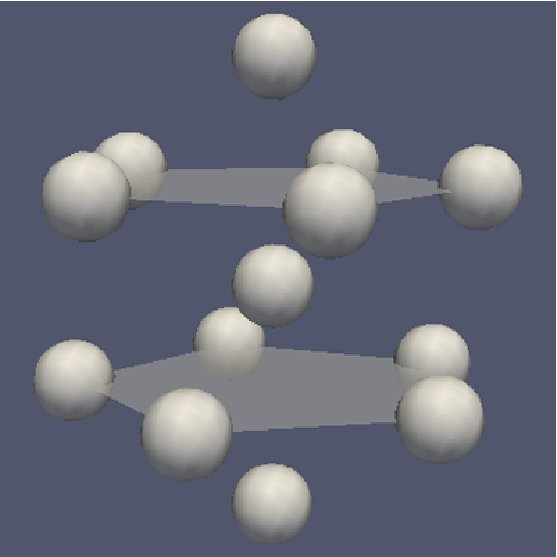
\includegraphics[width=\textwidth]{ico_13}\\
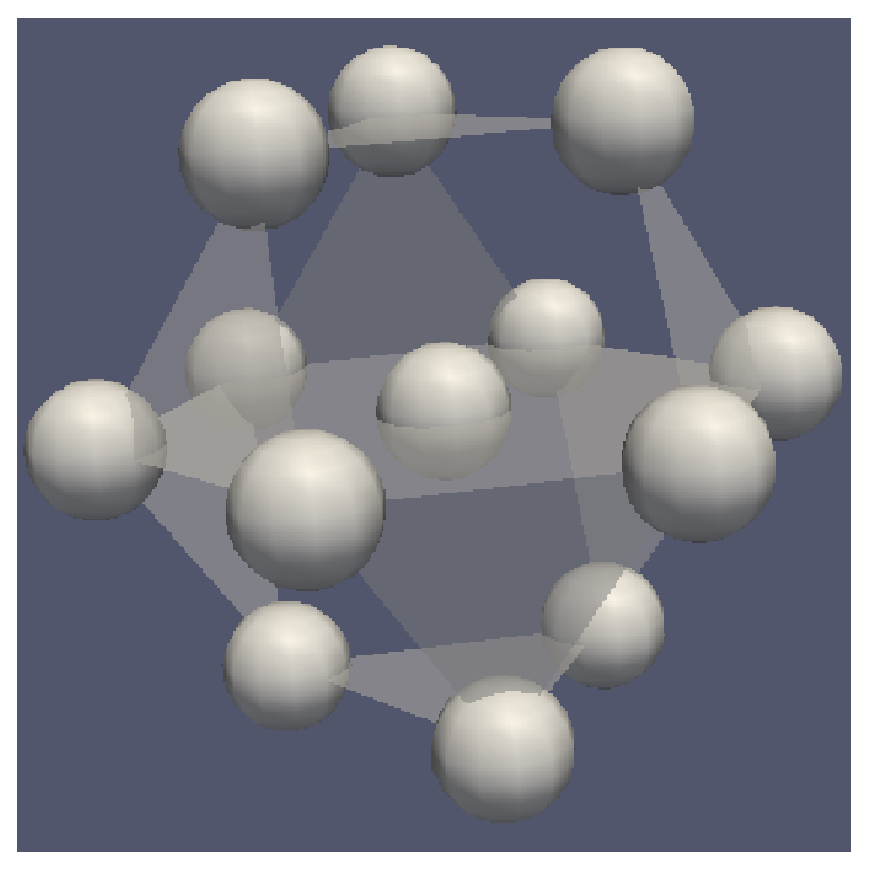
\includegraphics[width=\textwidth]{fcc_13}
\end{columns}
\end{block}
\structure{Single-particle colloidal experiments}\hfill \textit{\scriptsize Nature Commun. 2012}

\medskip
\tikzsetnextfilename{ico_dyn}\begin{tikzpicture}
	\begin{groupplot}[%
		group style = {
			group name=g,
			group size=2 by 1,
			horizontal sep = 3em
		},
		height=10em,%Tout est controlle par cette longueur
		width=0.35\columnwidth,
		label shift=-0.5em, %
		]
	\nextgroupplot[
		cycle list name=black white,
		every mark/.append style={scale=1.2},
		xlabel=$\phi$, xmin=0.49, xmax=0.58, xlabel near ticks,%
		xtick={0.5,0.53,...,0.6},%
		ylabel=$\xi/\xi_0$, ymax=10,
		ytick={2,4,6,8},
		legend pos=north west,%
		]
		\addplot+[only marks, mark=*, %
			every mark/.append style={fill=black, scale=1.2},
			error bars/.cd, y dir=both, y explicit relative,%
			] table[x index=0, y expr=\thisrowno{3}/0.126]{scale.xi};
		\addplot+[mark=none, forget plot, domain=0.49:0.58] {(0.6/x-1)^(-2.0/3.0)};
		\addplot+[only marks, mark=square, every mark/.append style={draw=gray, scale=1.2},] table[x index=0, y expr=\thisrowno{5}/0.216]{scale.xi};
		\legend{dynamic, crystalline};
	\nextgroupplot[
		ylabel={$\xi/\sigma$},
		ymax=1.9,
		xlabel={Pressure},
		ymin=0,
		xmin=8,
		xtick={9,13,...,25},]
	\pgfplotstableread{lengths}\lengths
	\addplot+[Main,every mark/.append style={fill=Main}] table[x index=0, y index=5]{\lengths} node[above left] {crystalline};
	\addplot+[Accent2,every mark/.append style={fill=Accent2}] table[x index=0, y index=4]{\lengths} node[above left] {icosahedral};
\end{groupplot}
%
\newdimen\mydima
\newdimen\mydimb
\pgfextracty{\mydima}{\pgfpointanchor{g c1r1}{north}}
\pgfextracty{\mydimb}{\pgfpointanchor{g c1r1}{south}}
\pgfmathsetlength{\mydima}{\mydima-\mydimb}
%
\begin{scope}[inner sep=0]
\node[anchor= south west] (mrco) at ($(g c2r1.right of south east)+(-\textwidth,0)$) {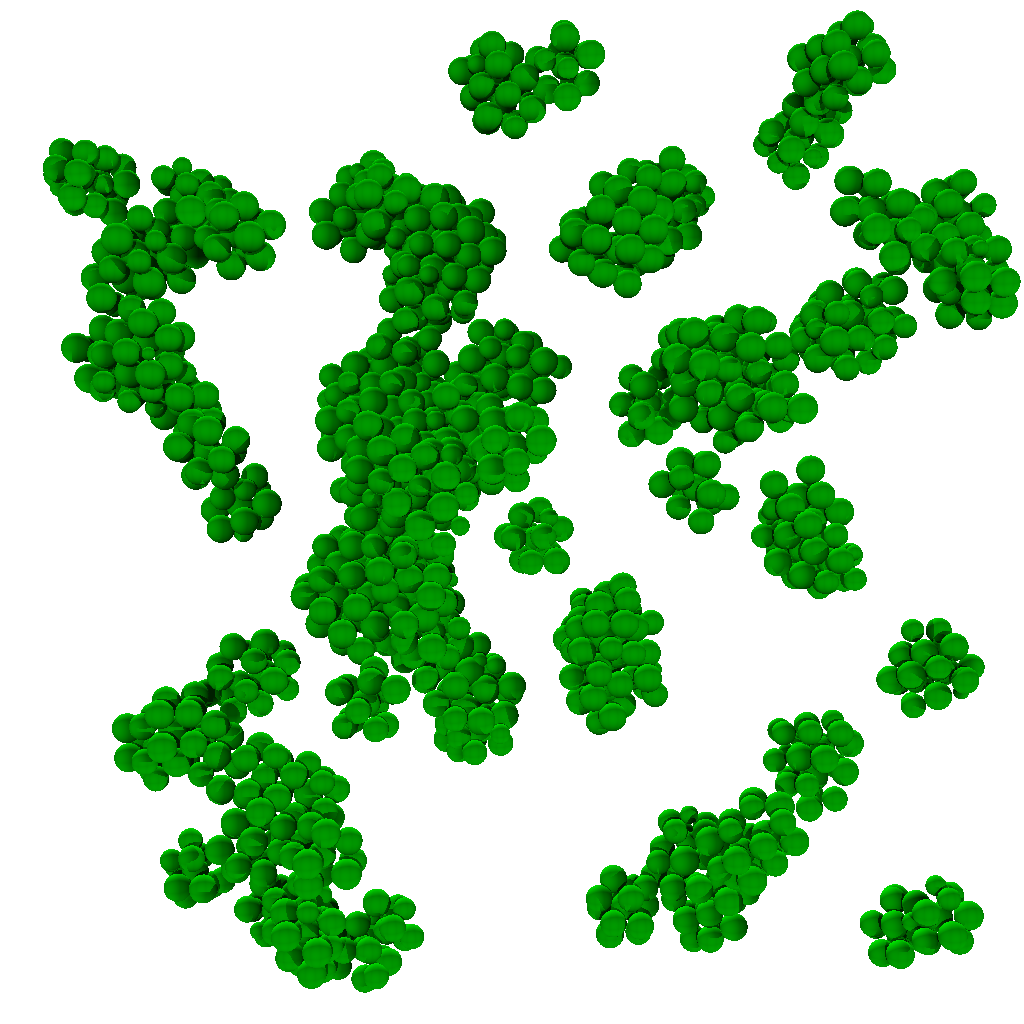
\includegraphics[height=\mydima]{mrco24_scale_go1_t040_t048.png}};
\node [below right=0 and 0.01\textwidth of mrco.north east] (slow) {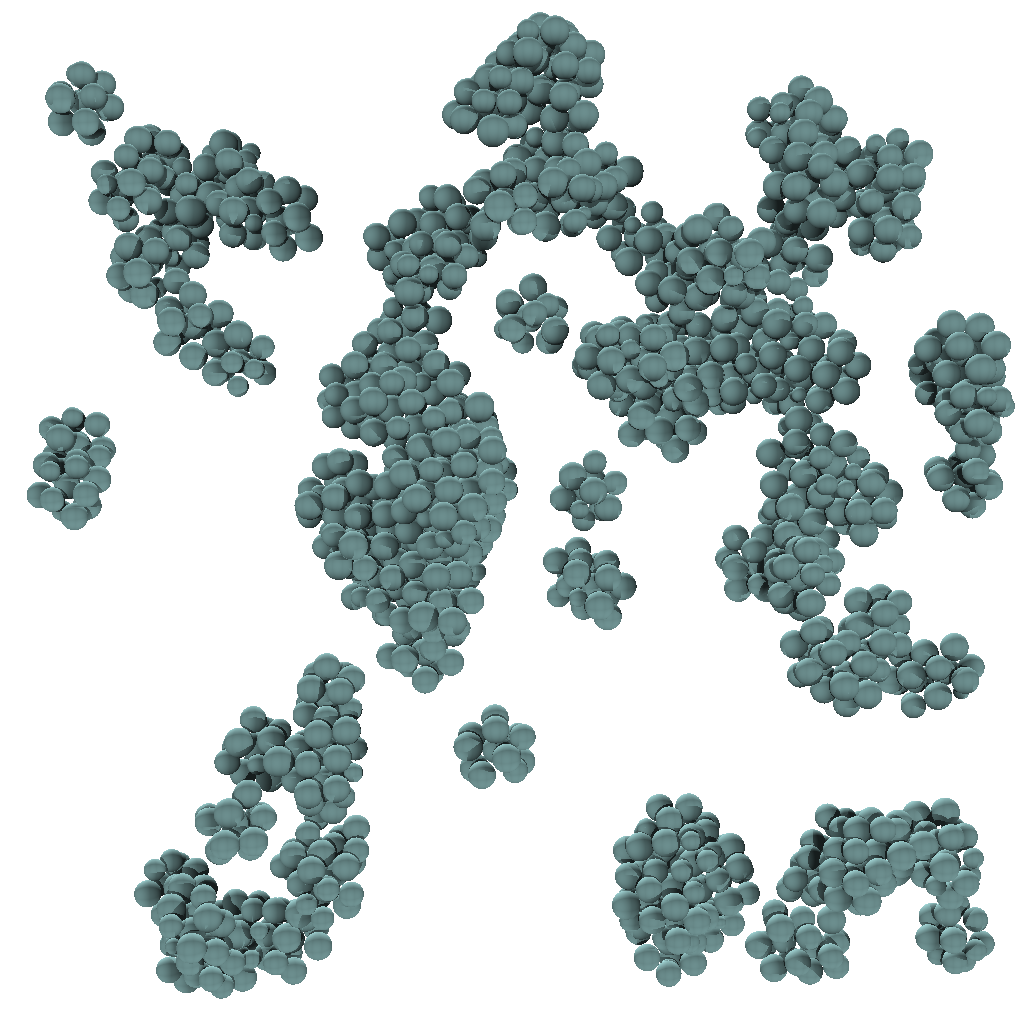
\includegraphics[height=\mydima]{cgsd_2tau.png}};
%labels
\begin{scope}[align=center]
	\node[below=0.2em of mrco, text width=\mydima] {crystal-like};
	\node[below=0.2em of slow, text width=\mydima]  {slow};
\end{scope}
\draw [help lines, step=0.25\mydima, shift=(mrco.south west)] (0, 0) grid (\mydima, \mydima);
	\draw [help lines, step=0.25\mydima, shift=(slow.south west)] (0, 0) grid (\mydima, \mydima);
\end{scope}
%\node[inner sep=0, draw, fit=(mrco) (g c2r1.outer south east) (g c1r1.outer south)]{};
\end{tikzpicture}
%\begin{scriptsize}
%Experiments \myfullcite{Leocmach2012}
%
%Simulations \myfullcite{Leocmach2013a}
%\end{scriptsize}

\end{frame}


\begin{frame}{Postdoc : Gelation mechanics}
%Colloidal gelation as arrested spinodal, but:\hfill\textit{\scriptsize Lu et al. Nature 2008}
%\begin{itemize}
%\item Gel structure shear-history dependent. Pre-shear $\rightarrow 0$?
%\item Hydrodynamic interactions. Can we forget about the solvent?
%\item[$\Rightarrow$] \textit{in situ} gelation under confocal microscope
%\end{itemize}
\begin{block}{Single-particle confocal microscopy experiments}
\begin{itemize}
\item Colloids as model atoms
\item Allow same analysis as simulations
\item On a real system
\end{itemize}
\end{block}


\bigskip
\structure{Mechanical tension prior bond breaking in aging gel}\hfill\textit{\scriptsize in prep.}

\medskip
\tikzsetnextfilename{breaking}\begin{tikzpicture}
	\matrix[
		matrix of nodes, inner sep=0, column sep=0.014\textwidth, 
		row sep=0.5em,
		] (m){
		\SI{0}{\minute} & \SI{16}{\minute} & \SI{22}{\minute} & \SI{30.5}{\minute} & \SI{31}{\minute} & \SI{90}{\minute} \\
		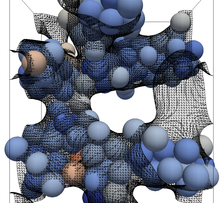
\includegraphics[width=0.155\textwidth]{breaking_particles_wireframe_t0000s.png}&
		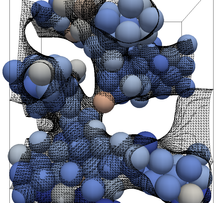
\includegraphics[width=0.155\textwidth]{breaking_particles_wireframe_t0032s.png}&
		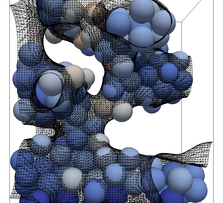
\includegraphics[width=0.155\textwidth]{breaking_particles_wireframe_t0043s.png}&
		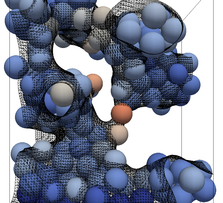
\includegraphics[width=0.155\textwidth]{breaking_particles_wireframe_t0061s.png}&
		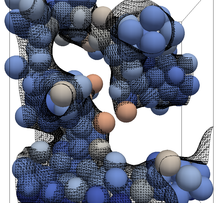
\includegraphics[width=0.155\textwidth]{breaking_particles_wireframe_t0062s.png}&
		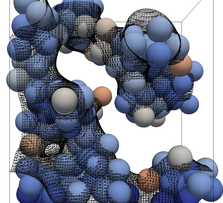
\includegraphics[width=0.155\textwidth]{breaking_particles_wireframe_t0180s.png}\\
		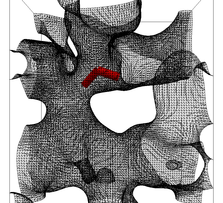
\includegraphics[width=0.155\textwidth]{breaking_wireframe_t0000s.png}&
		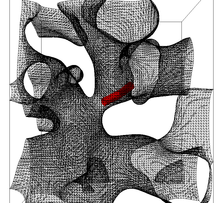
\includegraphics[width=0.155\textwidth]{breaking_wireframe_t0032s.png}&
		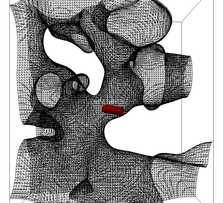
\includegraphics[width=0.155\textwidth]{breaking_wireframe_t0043s.png}&
		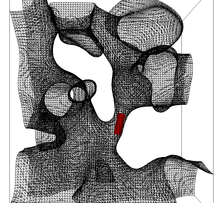
\includegraphics[width=0.155\textwidth]{breaking_wireframe_t0061s.png}&
		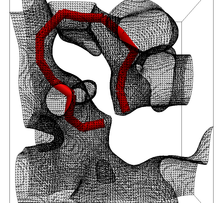
\includegraphics[width=0.155\textwidth]{breaking_wireframe_t0062s.png}&
		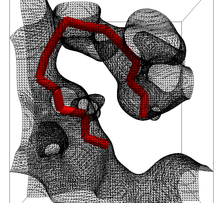
\includegraphics[width=0.155\textwidth]{breaking_wireframe_t0180s.png}\\
		};
\end{tikzpicture}

\end{frame}
